\documentclass[11pt]{article}

% =====================================================================
% XeLaTeX + Hebrew setup
% =====================================================================
\usepackage{fontspec}
\usepackage{polyglossia}
\setmainlanguage{hebrew}
\setotherlanguage{english}
\setmainfont{FreeSerif}
\newfontfamily\hebrewfont[Script=Hebrew]{FreeSerif}

% =====================================================================
% PACKAGES
% =====================================================================
\usepackage{amsmath}
\usepackage{amssymb}
\usepackage{graphicx}
\usepackage{float}
\usepackage{booktabs}
\usepackage{siunitx}
\usepackage{geometry}
\usepackage{indentfirst}
\usepackage{xcolor}
\usepackage{tcolorbox}
\tcbuselibrary{skins}

% =====================================================================
% PAGE GEOMETRY
% =====================================================================
\geometry{
  a4paper,
  top=2.5cm, bottom=2.5cm,
  left=2.5cm, right=2.5cm
}
\parskip 2mm

% =====================================================================
% FIGURE BOX — Option A
%
% Usage:
%   \begin{figbox}{כותרת האיור}
%     \includegraphics[width=0.96\textwidth]{figures/...}
%     \fcap{תופעה}{התאמה}{פרמטרים}{שגיאה}
%   \end{figbox}
% =====================================================================
\definecolor{boxblue}{RGB}{30, 60, 100}
\definecolor{capbg}{RGB}{245, 247, 252}

\newenvironment{figbox}[1]{%
  \begin{tcolorbox}[
    enhanced,
    colback=white,
    colframe=boxblue,
    coltitle=white,
    colbacktitle=boxblue,
    fonttitle=\bfseries\large,
    title={#1},
    top=6pt, bottom=6pt,
    left=6pt, right=6pt,
    toptitle=4pt, bottomtitle=4pt,
    lines before break=10,
  ]
  \centering
}{%
  \end{tcolorbox}
  \vspace{6pt}
}

\newcommand{\fcap}[4]{%
  \par\vspace{4pt}
  \noindent\colorbox{capbg}{%
    \begin{minipage}{0.97\textwidth}
      \vspace{4pt}
      \textbf{(א) תופעה:} #1\par\smallskip
      \textbf{(ב) התאמה:} #2\par\smallskip
      \textbf{(ג) פרמטרים:} #3\par\smallskip
      \textbf{(ד) שגיאה:} #4
      \vspace{4pt}
    \end{minipage}%
  }%
}

% =====================================================================
% DOCUMENT
% =====================================================================
\begin{document}

% ----- Title block ---------------------------------------------------
\begin{center}
  {\LARGE \textbf{(77335) מעבדה בפיזיקה ב-2 $|$ ניסוי 1: כאוס}}\\
  \vspace{0.5cm}
  {\large שקד סוקניק \quad ת"ז: 313566895}\\
  {\large ניר כהן \quad ת"ז: 209720838}\\
  \vspace{0.3cm}
  {\normalsize \today}
\end{center}

\hrule
\vspace{0.5cm}

% =====================================================================
% §1  מטרת הניסוי
% =====================================================================
\section*{מטרת הניסוי}

ניסוי זה בוחן את התנהגות הדיודה 1N4005 דרך מדידת עקומת ה-I-V וקיבול המעבר,
ואת מעגל ה-RLD כמערכת דינמית לא-לינארית המפגינה הכפלת-מחזור ומעבר לכאוס.
המטרה היא לאמת את משוואת Shockley, למדוד את תלות $C_j(V)$, ולאפיין את מפת
הבפורקציה בהתאם לתיאוריה האוניברסלית של פייגנבאום.

\vspace{0.5cm}

% =====================================================================
% §2  מערכת הניסוי
% =====================================================================
\section*{מערכת הניסוי}

\textbf{חלק 1 — אפיון דיודה:}
מחולל פונקציות מחובר בטור עם נגד $R = \SI{470}{\ohm}$ ודיודה 1N4005.
ערוץ 1 (Ch1) מדד את מתח קצות הדיודה; ערוץ 2 (Ch2) את מתח יציאת המחולל.
הזרם חושב כ-$I_D = (V_{\text{Ch2}} - V_{\text{Ch1}}) / R$.

\textbf{חלק 2 — מעגל RLD:}
נוסף סליל $L = \SI{100}{\milli\henry}$ בטור. גל נושא בתדר $\approx\SI{34}{\kilo\hertz}$
עם מודולציית AM בתדר $\SI{0.7}{\hertz}$ ושיא $\SI{7}{\volt}$ שימש לסריקה רציפה
של משרעת הכניסה.

\vspace{0.5cm}

% =====================================================================
% §3  תוצאות
% =====================================================================
\section*{תוצאות}

% ----- Figure 1: Discrete I-V ----------------------------------------
\begin{figbox}{איור 1 — עקומת I-V בדידה (גל ריבועי)}
  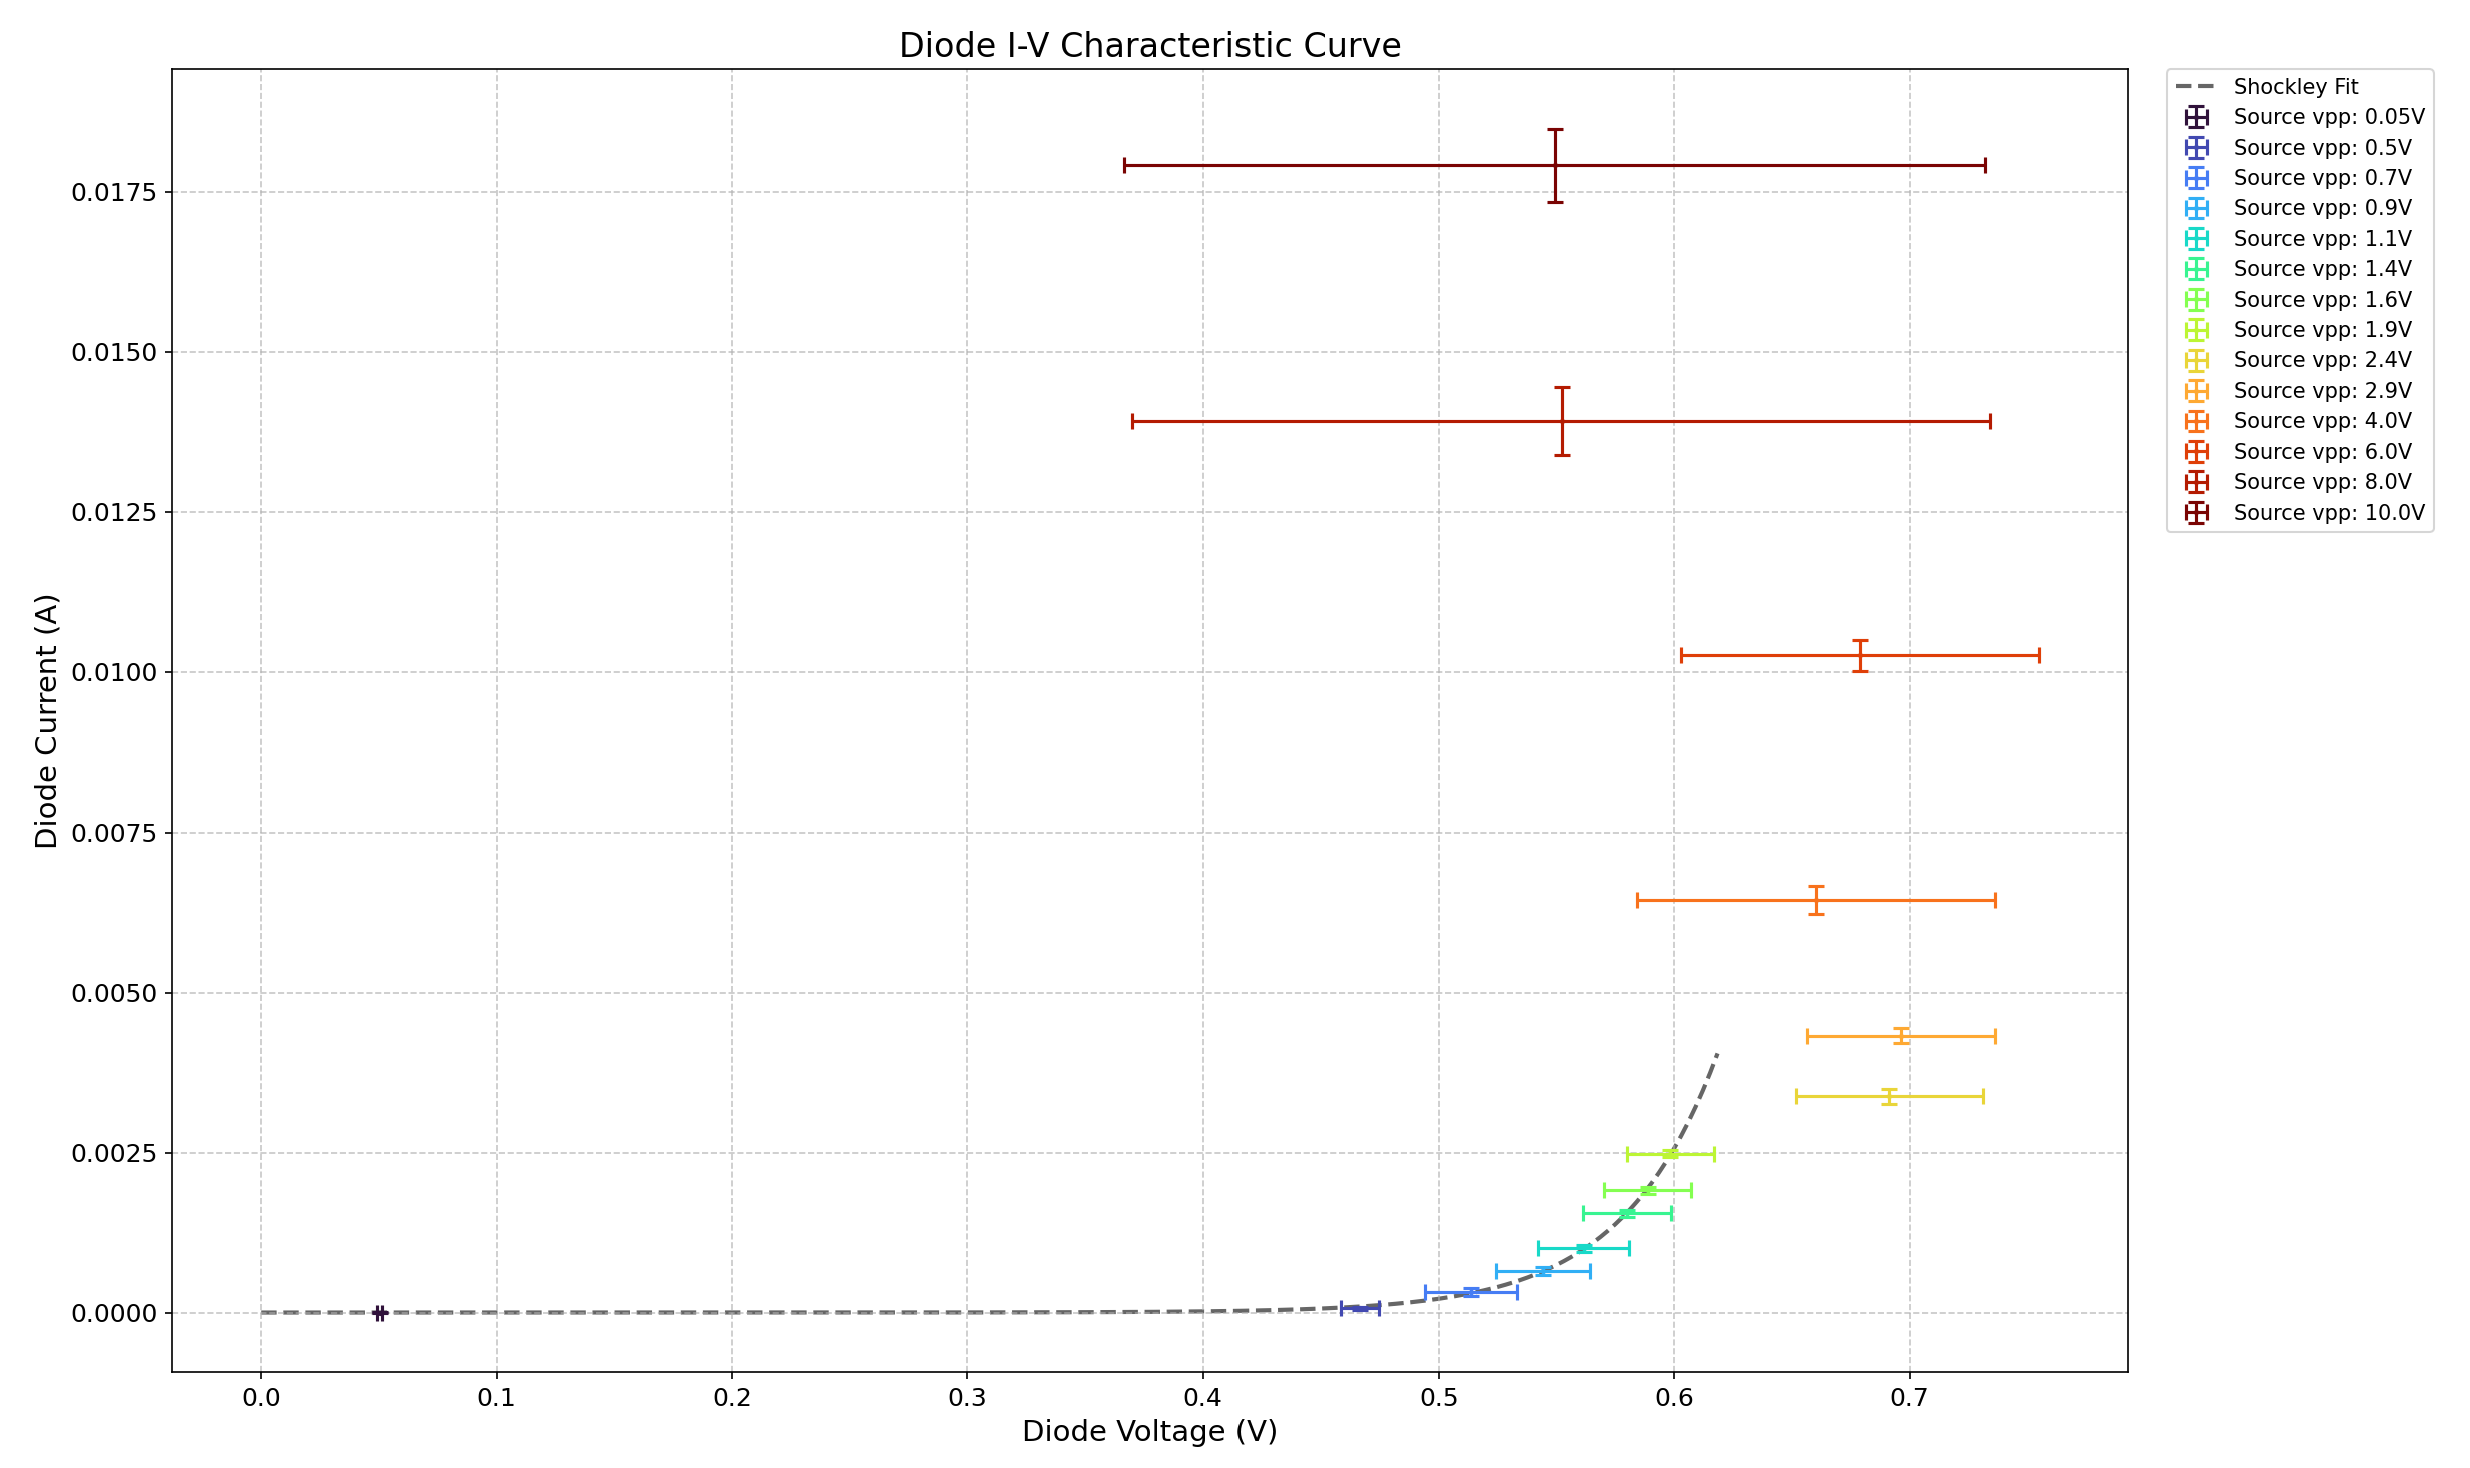
\includegraphics[width=0.96\textwidth]{figures/graph1IV.png}
  \fcap
    {עקומת מאפייני I-V של דיודת 1N4005 הנמדדת בגל ריבועי ($R = \SI{470}{\ohm}$).
     כל נקודה מייצגת ממוצע של דגימות בפלטו. נקודות עם $V_{pp} \geq \SI{6}{\volt}$
     סוטות מהמודל עקב התנגדות סדרתית בזרמים גבוהים ואינן כלולות בהתאמה.}
    {$I = I_S\!\left(e^{V_D/nV_T}-1\right)$,\quad $V_T = \SI{25.85}{\milli\volt}$}
    {$n = \text{TODO}$,\quad $I_S = \text{TODO}\ \si{\ampere}$}
    {קוונטיזציית ADC $\approx \SI{80}{\milli\volt}$ (2\,V/div, 8-bit);
     זרם: $\sigma_I = \sigma_{\Delta V}/\SI{470}{\ohm}$}
\end{figbox}

% ----- Figure 2: Continuous I-V (triangle) ---------------------------
\begin{figbox}{איור 2 — עקומת I-V רציפה (גל משולש)}
  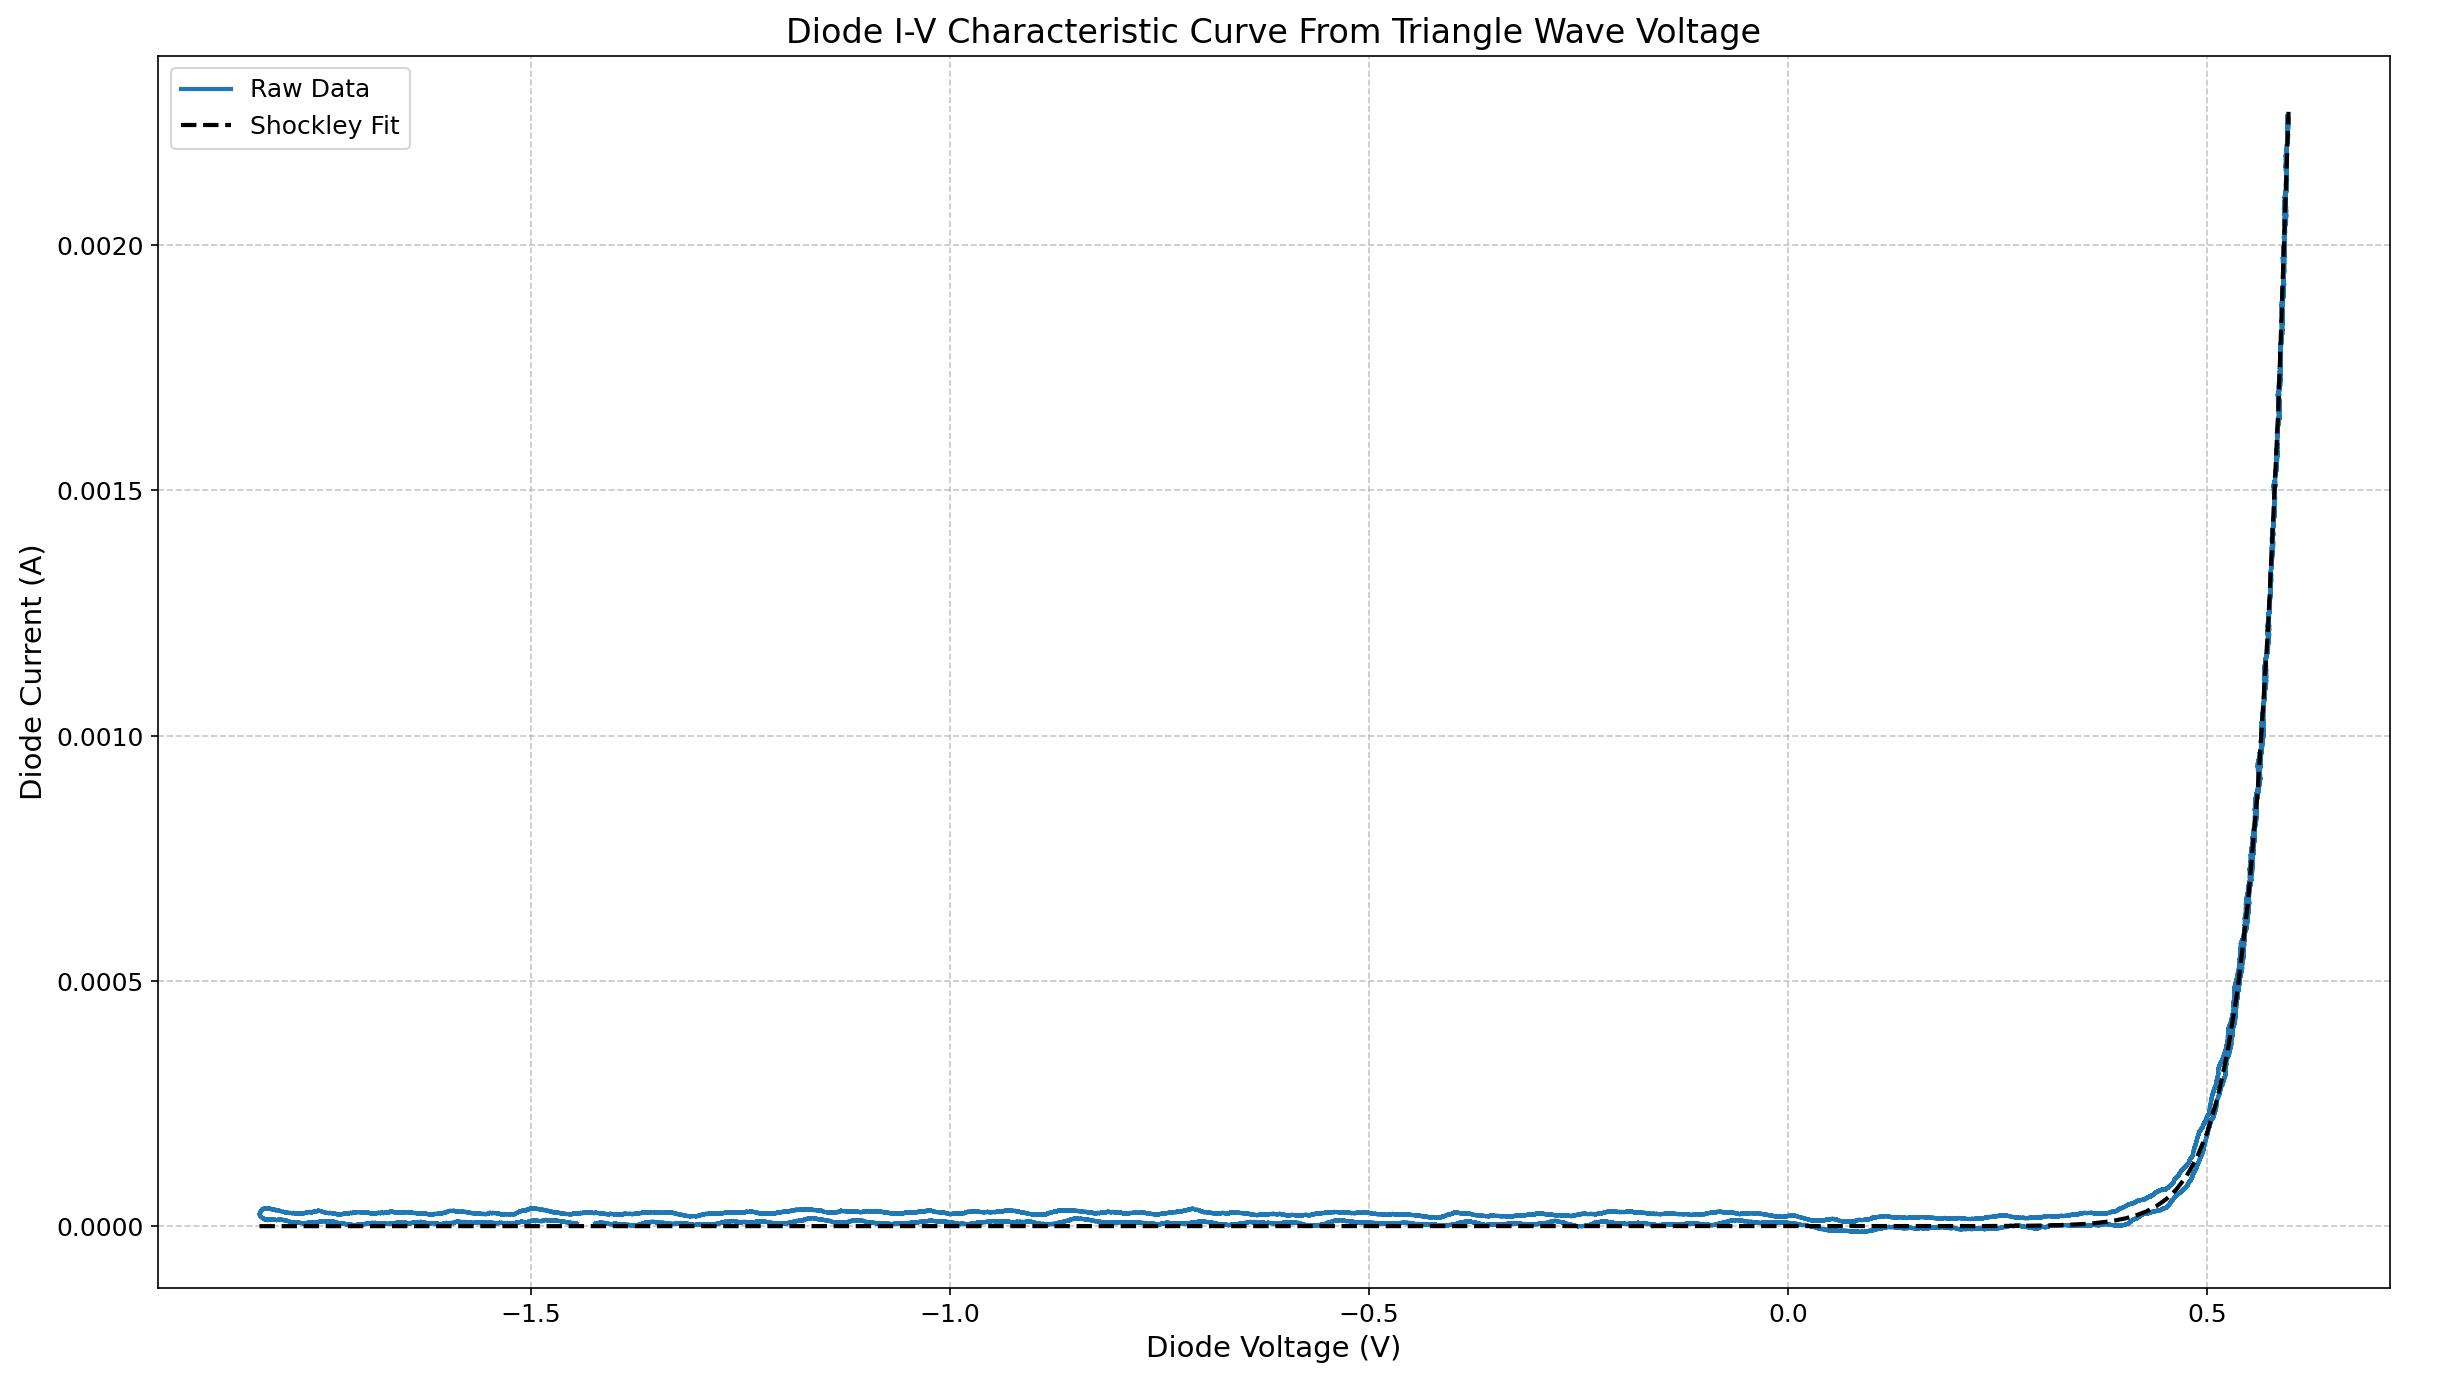
\includegraphics[width=0.96\textwidth]{figures/graph2IV_Triangle.png}
  \fcap
    {עקומת מאפייני I-V של דיודת 1N4005 הנמדדת בגל משולש. הרצועה הכחולה הרחבה
     משקפת את שני כיווני הסריקה (עולה ויורדת). היסט חיובי קבוע של
     $\approx \SI{0.3}{\milli\ampere}$ בהטיה הפוכה הוא ארטיפקט של רמת בסיס ה-ADC.}
    {$I = I_S\!\left(e^{V_D/nV_T}-1\right)$, מותאם לאזור הטיה קדמית ($V_D > \SI{0.3}{\volt}$)}
    {$n = \text{TODO}$,\quad $I_S = \text{TODO}\ \si{\ampere}$}
    {הרצועה הנראית לעין משקפת רעש; אין פס שגיאה פורמלי.}
\end{figbox}

% ----- Figure 3: C(V) ------------------------------------------------
\begin{figbox}{איור 3 — קיבול מעבר $C_j(V)$}
  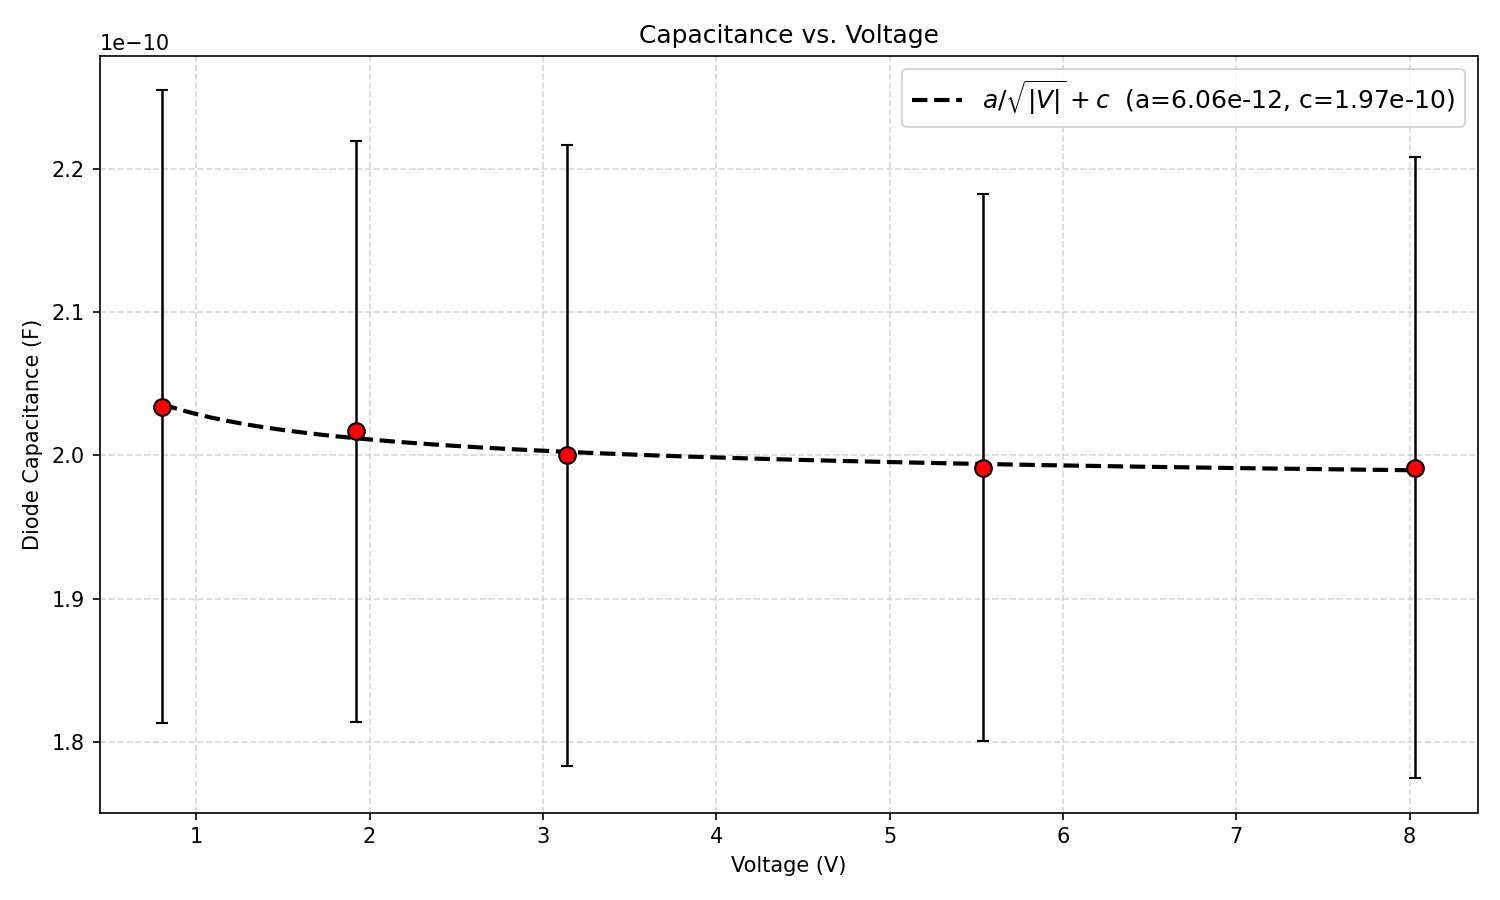
\includegraphics[width=0.96\textwidth]{figures/graph3C_V.png}
  \fcap
    {קיבול מעבר דיודת 1N4005 פוחת עם עליית המתח ההפוך, בהתאם לתיאוריית שכבת
     הניגוד. סך הוריאציה הנמדדת $\approx \SI{4.5}{\pico\farad}$ על בסיס
     $\approx \SI{200}{\pico\farad}$, מה שמצביע על ריסון חלש של ההתאמה.}
    {$C_j(V) = a/\!\sqrt{|V|} + c$}
    {$a = \text{TODO}\ \si{\farad\cdot\volt^{1/2}}$,\quad $c = \text{TODO}\ \si{\farad}$}
    {אופקי: קוונטיזציית ADC; אנכי ($\sigma_\tau \to \sigma_C = \sigma_\tau/R$): טרם נוסף.}
\end{figbox}

% ----- Figure 4: Discrete bifurcation --------------------------------
\begin{figbox}{איור 4 — דיאגרמת בפורקציה בדידה}
  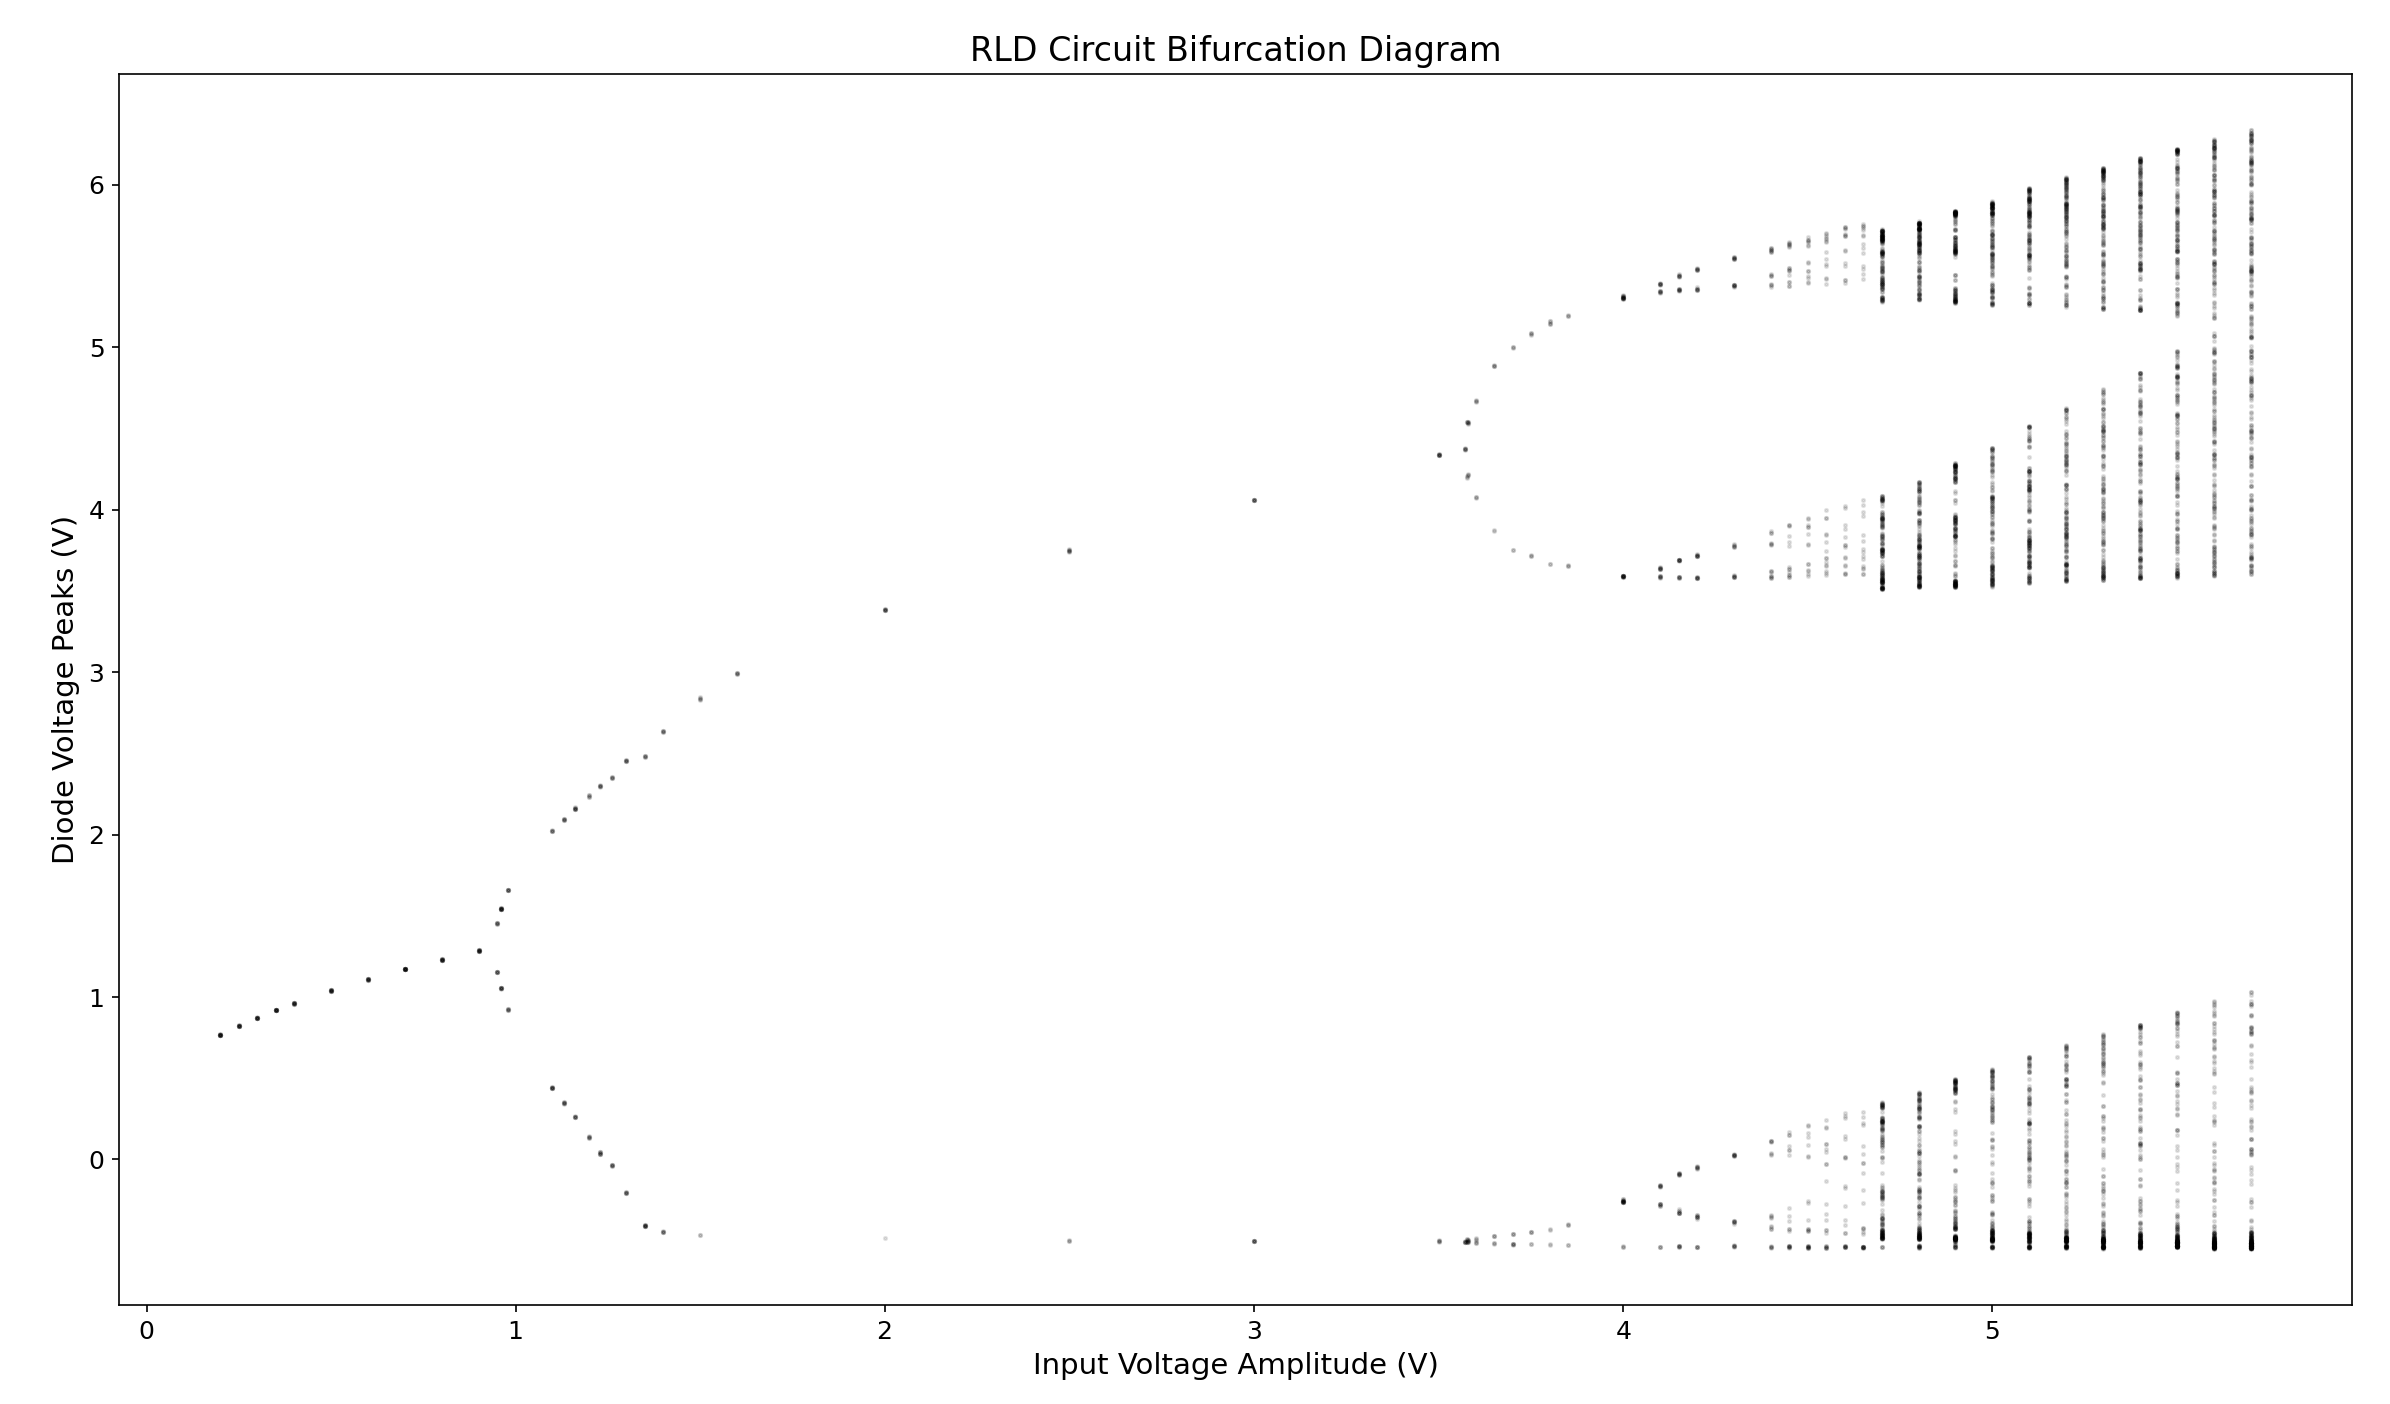
\includegraphics[width=0.96\textwidth]{figures/graph4_bifrocation.png}
  \fcap
    {דיאגרמת בפורקציה בדידה של מעגל RLD ($R=\SI{470}{\ohm}$, $L=\SI{100}{\milli\henry}$,
     דיודת 1N4005). מוצגת מפלת הכפלת-מחזור 1→2→4→כאוס ככל שמשרעת הכניסה עולה.
     גוון האפור — TODO (לבדוק ב-\textenglish{get\_cycles.py}).}
    {אין התאמה}
    {אין}
    {קוונטיזציית ADC $\approx \SI{80}{\milli\volt}$ (2\,V/div, 8-bit); פסי שגיאה — יש להוסיף.}
\end{figbox}

% ----- Figure 5: Continuous bifurcation ------------------------------
\begin{figbox}{איור 5 — מפת בפורקציה רציפה (AM)}
  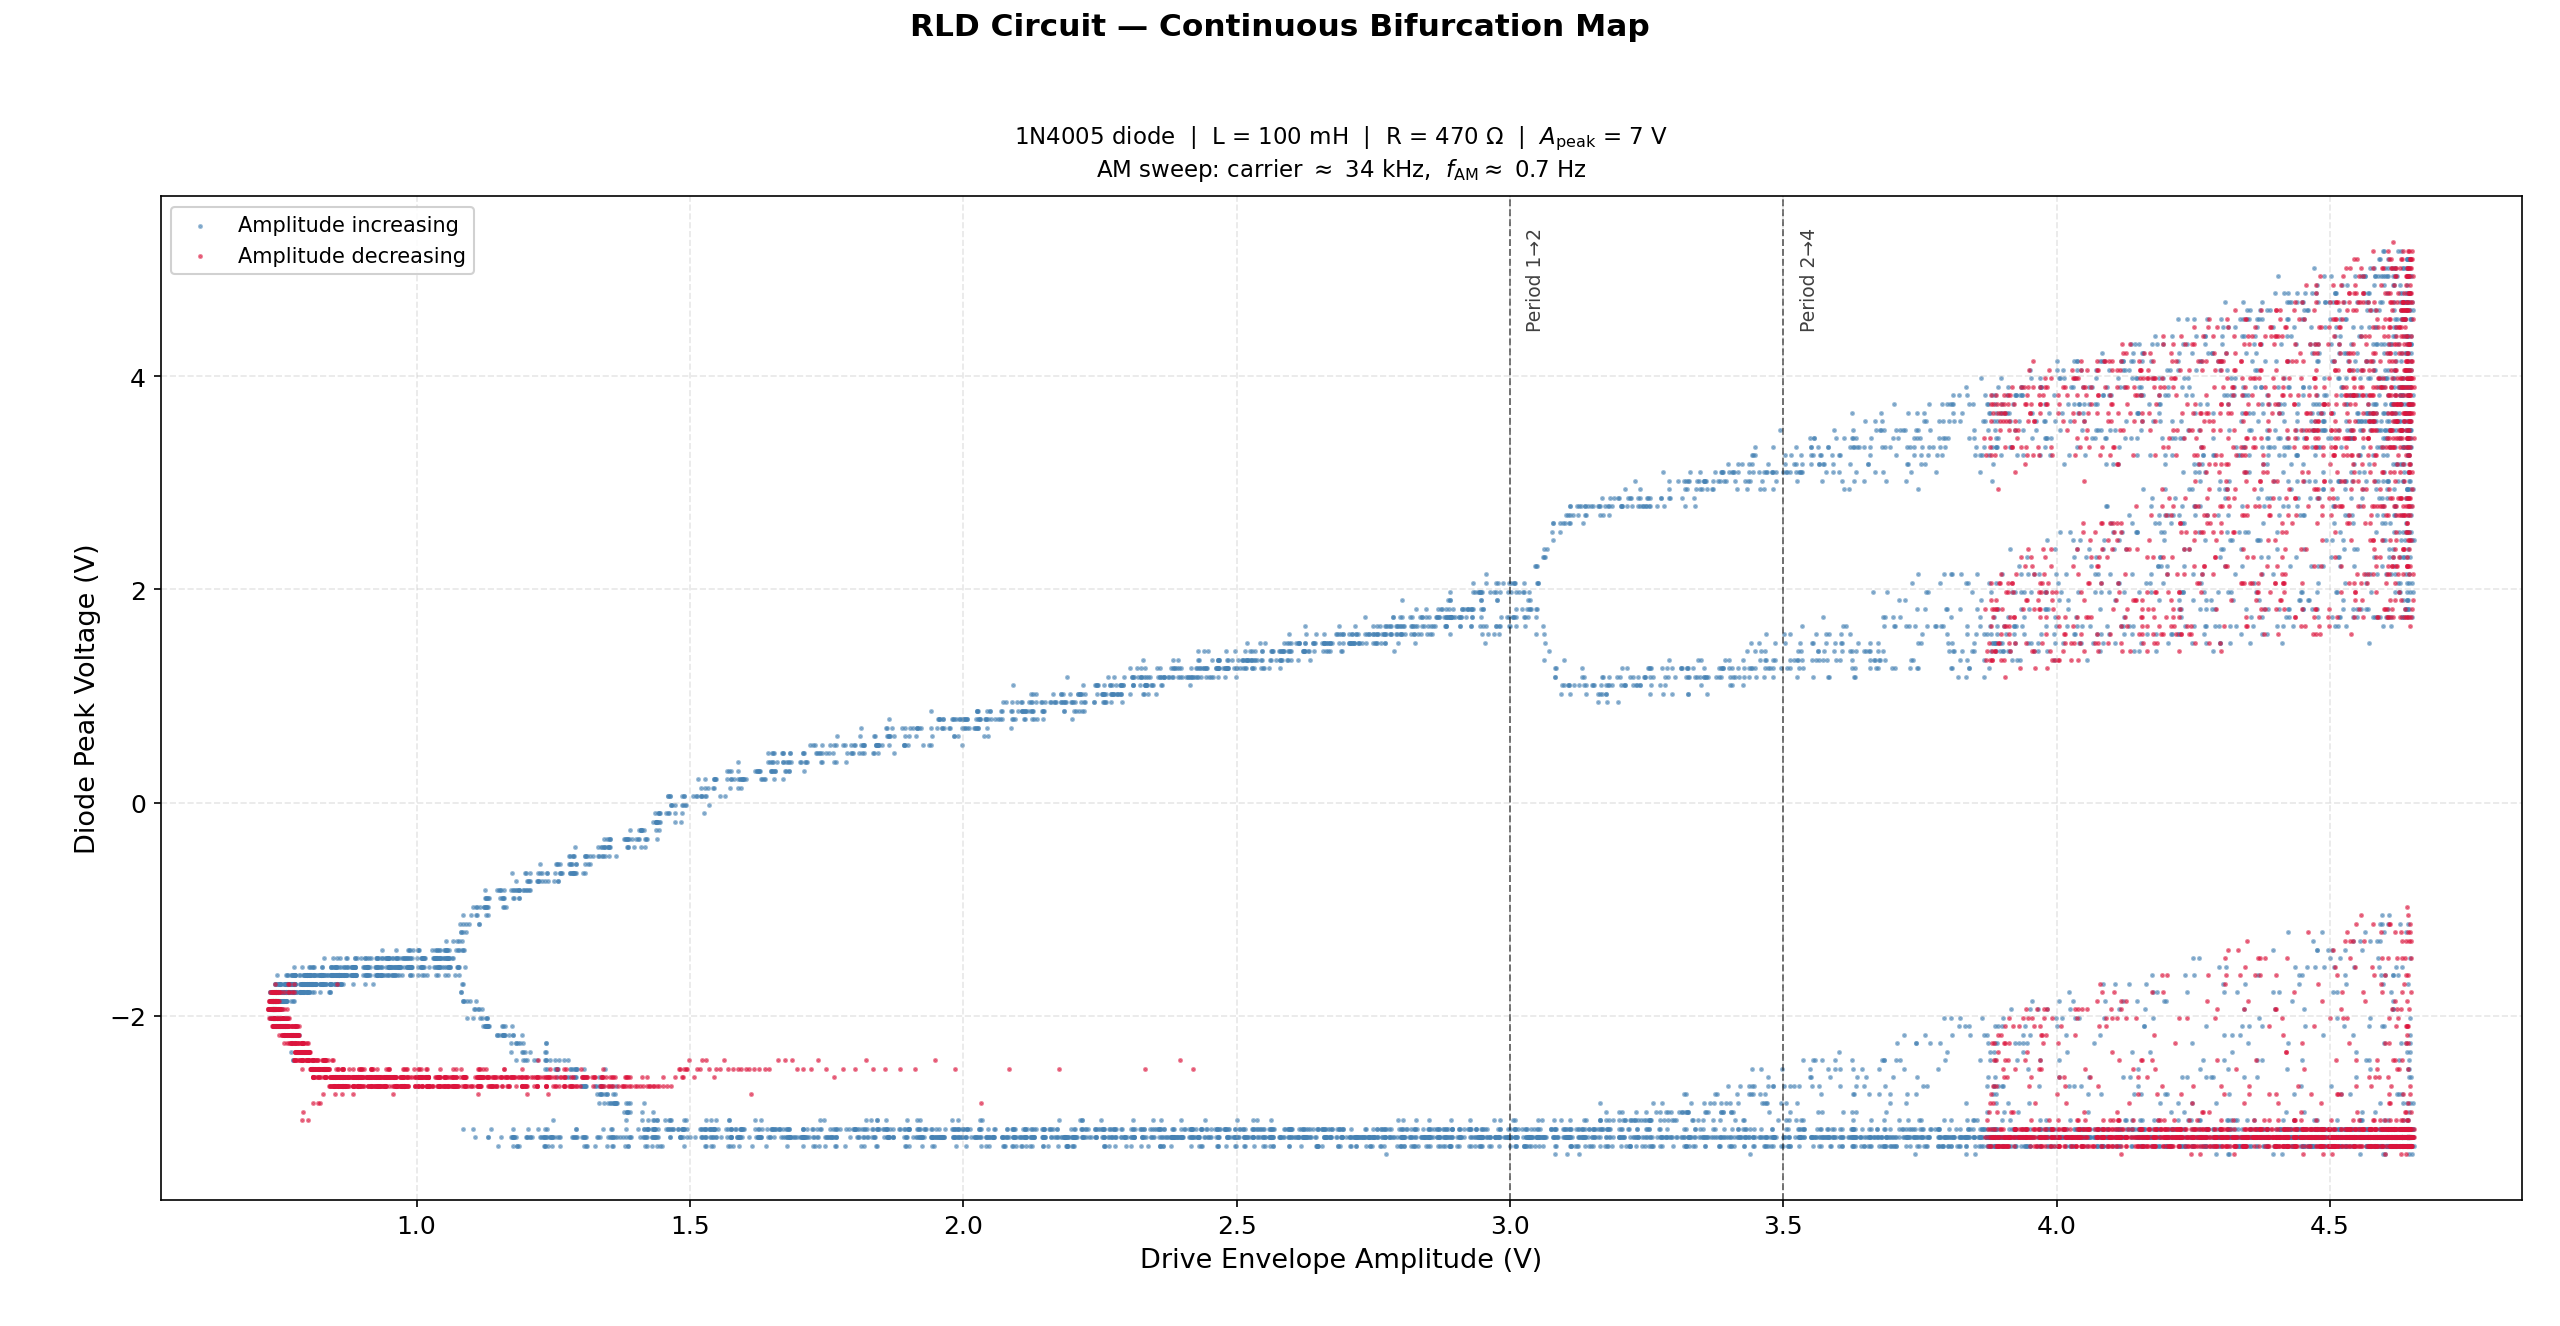
\includegraphics[width=0.96\textwidth]{figures/graph5_bifurcation_cont_triangle.png}
  \fcap
    {מפת בפורקציה רציפה של מעגל RLD (נושאת $\approx\SI{34}{\kilo\hertz}$,
     $f_{AM}\approx\SI{0.7}{\hertz}$, שיא $\SI{7}{\volt}$). כחול = משרעת עולה,
     אדום = יורדת; ההפרדה מצביעה על היסטרזיס. ענף עליון: שיאי הטיה קדמית;
     ענף תחתון: שיאי הטיה הפוכה (קבועים, $\approx\SI{-3.5}{\volt}$).}
    {אין התאמה}
    {קווי מעבר (הערכה חזותית, $\pm\SI{0.1}{\volt}$):
     $1\!\to\!2 \approx \SI{3.0}{\volt}$,\quad $2\!\to\!4 \approx \SI{3.5}{\volt}$}
    {קוונטיזציית ADC $\approx \SI{80}{\milli\volt}$.}
\end{figbox}

\vspace{0.5cm}

% =====================================================================
% §4  דיון
% =====================================================================
\section*{דיון}

% TODO

\vspace{0.5cm}

% =====================================================================
% §5  נספחים
% =====================================================================
\section*{נספחים}

% TODO

\end{document}
